\subsection{Intro}
    \subsubsection{QS algorithm}
    \begin{definition}
        \begin{lstlisting}[language=Python, caption={Quicksort Algorithm Pseudocode}]
            Quicksort (list in, int left, int right)
                pivot = Partition(in, left, right)
                if (pivot > left)
                    Quicksort(in, left, pivot)
                if (pivot < right)
                    Quicksort(in, pivot + 1, right)
        \end{lstlisting}
    \end{definition}

    \subsubsection{Partition}
    \begin{definition}
        \begin{lstlisting}[language=Python, caption={Partition Function Pseudocode}]
            int Partition (in, left, right)
                ls = left
                pivot = in(left)
                for i = left + 1 to right
                    if (in(i) <= pivot)
                        ls = ls + 1
                        swap(in(i), in(ls))
                swap(in(left), in(ls))
                return ls
        \end{lstlisting}
    \end{definition}

    \begin{intuition}
        \customFigure[1]{00_Images/Quicksort_Example1.png}{Quicksort example.}          
    \end{intuition}

\subsection{QS basic analysis}
    \subsubsection{QS best case}
    \begin{definition}
        The array is always split exactly in half, leading to a balanced partition. The recurrence relation for quicksort in this scenario is:

        \begin{equation*}
            T(n) = 2T\left(\frac{n}{2}\right) + \Theta(n)
        \end{equation*}

        \begin{center}
            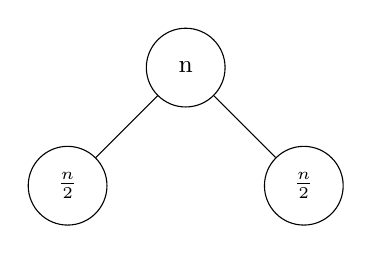
\begin{tikzpicture}[level distance=1.5cm, sibling distance=3cm, every node/.style={circle, draw, minimum size=1cm, font=\small}]
                % Root level for BC
                \node {n}
                    % First level of BC partitioning
                    child {node {$\frac{n}{2}$}}
                    child {node {$\frac{n}{2}$}};
            \end{tikzpicture}
        \end{center}

        \noindent Now using the Master Theorem:
        \begin{equation*}
        T(n) = \Theta(n \log n)
        \end{equation*}
    \end{definition}

    \subsubsection{QS worst case}
        \begin{definition}
            The array is already sorted (or reverse sorted) and we choose the first or last element as the pivot, the recurrence relation for quicksort is:

            \[
            T(n) = T(n-1) + \Theta(n)
            \]

            \begin{center}
                % Worst Case (WC) Tree
                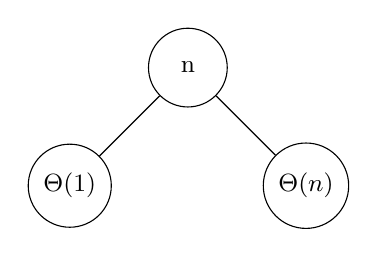
\begin{tikzpicture}[level distance=1.5cm, sibling distance=3cm, every node/.style={circle, draw, minimum size=1cm, font=\small}]
                    % Root level for WC
                    \node {n}
                        % First level of WC partitioning
                        child {node {$\Theta(1)$}}
                        child {node {$\Theta(n)$}};
                \end{tikzpicture}
            \end{center}

            \noindent This recurrence relation expands as follows:

            \begin{align*}
                T(n) &= T(n-1) + \Theta(n) \\
                    &= \left(T(n-2) + \Theta(n-1)\right) + \Theta(n) \\
                    &= \left(T(n-3) + \Theta(n-2)\right) + \Theta(n-1) + \Theta(n) \\
                    &= \cdots \\
                    &= \Theta\left(\sum_{i=1}^{n} i\right) \\
                    &= \Theta\left(\frac{n(n+1)}{2}\right) \\
                    &= \Theta(n^2)
            \end{align*}
        \end{definition}

    \subsubsection{QS average case}
    \begin{definition}
        In the average case, the recurrence relation for quicksort can be expressed as:

        \[
        T(n) = T\left(\frac{n}{10}\right) + T\left(\frac{9n}{10}\right) + \Theta(n)
        \]

        \noindent We can visualize this with a recursion tree:

        \customFigure[0.5]{00_Images/Quicksort_Average.png}{Quicksort average case in which each level is derived by subbing in the $T(\#)$ back into the equation above.}          

        \noindent Based on the recursive tree structure and the average-case recurrence relation, we can derive the time complexity as follows:

        \[
        T(n) = h \cdot \Theta(n)
        \]

        \noindent Now, let's calculate the height \( h \) of the tree:

        \[
        \left(\frac{9}{10}\right)^h n = 1
        \]

        \[
        h = \log_{10/9}(n) 
        \]

        \noindent Substituting this back into the overall complexity:

        \begin{align*}
        T(n) &= h \cdot \Theta(n) \\
            &= \log_{10/9}(n) \cdot \Theta(n) \\
            &= \Theta(n \log n)
        \end{align*}

    \end{definition}

\subsection{Worst-case (formal)}
    \begin{definition}
        The worst-case recurrence relation for quicksort can be expressed as:

        \[
        T(n) = \text{time to QS n-elements} = \max_{1 \leq q \leq n-1} \{ T(q) + T(n-q) \} + \Theta(n)
        \]

        \begin{center}
            % Worst Case (WC) Tree
            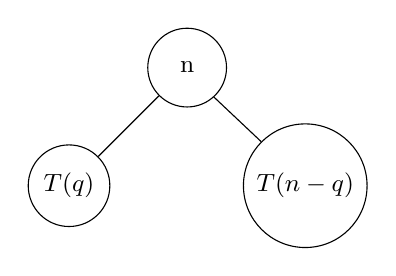
\begin{tikzpicture}[level distance=1.5cm, sibling distance=3cm, every node/.style={circle, draw, minimum size=1cm, font=\small}]
                % Root level for WC
                \node {n}
                    % First level of WC partitioning
                    child {node {$T(q)$}}
                    child {node {$T(n-q)$}};
            \end{tikzpicture}
        \end{center}

        % STOPPED HERE.
        \noindent We use substitution to show that \( T(n) \leq cn^2 \) for some constant \( c \).
        \begin{enumerate}
            \item Guess \( T(n) \leq cn^2 \).
            \item 
        \end{enumerate}
        \begin{align*}
            T(n) &\leq \max_{1 \leq q \leq n-1} \left\{ cq^2 + c(n-q)^2 \right\} + \Theta(n) \quad \text{(Achieves max at } q = 1 \text{ or } q = n-1 \text{)} \\
                 &= c \max_{1 \leq q \leq n-1} \left\{ q^2 + (n-q)^2 \right\} + \Theta(n) \quad \text{(As second derivative is positive, plug } q = 1 \text{)} \\
                 &\leq cn^2 - 2c(n-1) + \Theta(n) \quad \text{(We can pick a large } c \text{ to dominate the constant } \Theta(n)) \\
                 &\leq cn^2
        \end{align*}

        \noindent Therefore, using the substitution method, we can show that \( T(n) \leq cn^2 \), confirming that the worst-case time complexity of the quicksort algorithm is \( O(n^2) \).
    \end{definition}

\subsection{Randomized QS} 
    \subsubsection{Motivation for randomized QS}
    \begin{example}
        \begin{center}
            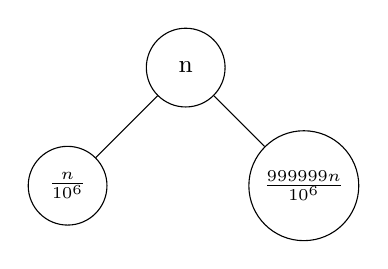
\begin{tikzpicture}[level distance=1.5cm, sibling distance=3cm, every node/.style={circle, draw, minimum size=1cm, font=\small}]
                % Root level
                \node {n}
                    % First level of partitioning
                    child {node {$\frac{n}{10^6}$}}
                    child {node {$\frac{999999n}{10^6}$}};
            \end{tikzpicture}
        \end{center}
        
        \noindent In this example, the array of size \( n \) is split into highly unbalanced sub-arrays:
        \begin{itemize}
            \item One sub-array is \( \frac{n}{10^6} \), very small compared to \( n \).
            \item The other sub-array is \( \frac{999999n}{10^6} \), almost the entire size of \( n \).
        \end{itemize}
        \vspace{1em}

        \noindent This unbalanced split may lead to increased recursion depth and higher running times, potentially reaching the worst-case \( O(n^2) \) complexity.
        \vspace{1em}

        \textbf{Motivation for Randomized QS:}
        \begin{itemize}
            \item Avoiding worst-case scenarios
            \item Ensuring balanced splits
            \item Works against sorted and reverse sorted arrays.
        \end{itemize}
    \end{example}

    \subsubsection{Random partition}
    \begin{definition}
        \begin{lstlisting}[language=Python, caption={Rand-Partition Function Pseudocode}]
            Rand-Partition (list in, left, right)
                i = random(left, right)
                swap(in(left), in(i))
                return Partition(in, left, right)
        \end{lstlisting}
    \end{definition}

